\documentclass[conference]{IEEEtran}
\usepackage[T1]{fontenc}
\usepackage{amsmath,amssymb,booktabs,array,graphicx}
\usepackage{algorithm,algpseudocode}
\usepackage{tikz}
\usetikzlibrary{arrows.meta,positioning}
\usepackage[hidelinks]{hyperref}
\usepackage{url,cite,balance}
\graphicspath{{figures/}}
\newcommand{\code}[1]{\texttt{#1}}
\pagestyle{plain}
\title{Recovering Blocked Agent Skills Without Prepared Replacements:\\A Study of State-Aware Continuations}
\author{\IEEEauthorblockN{Victor Cao}\IEEEauthorblockA{University of Auckland\\Auckland, New Zealand\\xcao541@aucklanduni.ac.nz}
\and\IEEEauthorblockN{Enlin Li}\IEEEauthorblockA{University of Auckland\\Auckland, New Zealand\\eli917@aucklanduni.ac.nz}}
\begin{document}
\maketitle\thispagestyle{plain}\raggedbottom
\begin{abstract}
Blocking a malicious agent Skill can protect resources while leaving the user's task unfinished. Recovery becomes harder when no prepared replacement exists and some actions have already happened. We study bounded continuation construction under fixed permissions. A residual effect contract combines unfinished task goals, reusable values, attacker-created dependencies, and confirmed or uncertain side effects. A constructor proposes a continuation; a common executable checker returns counterexamples before deployment. We evaluate six held-out synthetic task structures, varying inputs, partial execution, faults, strong controls and component ablations with GPT-6 Luna and GPT-4.1 mini. With shared transport normalization, the method safely completes 55/72 and 51/72 episodes, respectively. Ordinary Luna repair also completes 55/72, but requires 103 model requests rather than 31. Shared operand guidance improves replanning but leaves a completion gap. However, a source-free deterministic compiler completes all 20 feasible matched cases, and removing several proposed components does not reduce completion. Forty-three accepted programs fail fresh inputs. These findings support explicit state constraints and reduced model use in this finite setting, while limiting claims about novel synthesis, component necessity and real-world Skill security.
\end{abstract}

\begin{IEEEkeywords}
agent Skill security, safe recovery, program construction, side effects, executable evaluation
\end{IEEEkeywords}
\section{Introduction}
Agent Skills package instructions and helper code so that an agent can perform a reusable task. A reporting Skill, for example, may read a table, calculate totals, write a report and send it to a named recipient. This is useful because the user need not describe each tool call. It also creates a security problem. A malicious package can insert an unrelated credential read, mix private data into a legitimate message, or make the useful work depend on a forbidden action. Studies of malicious Skills and Skill-file injection show why package content should not receive the same trust as the user's request~\cite{liu,skillinject}.

An external gateway can block an action that violates a trusted policy. Blocking is necessary, but it does not by itself finish the user's task. If the gateway stops a credential read in the middle of report generation, the report may remain incomplete. Simply removing that read can also fail: later code may use the missing value, or a condition may make the final send depend on it. The malicious code has created a dependency, but that dependency does not give it permission to read the credential.

Recovery is harder once some useful work has already happened. Suppose the report was written before the block. Replaying the whole Skill can repeat the write. Suppose the report was sent but its acknowledgement was lost. Sending again can produce a duplicate; assuming success can leave the task incomplete when the first send did not happen. A recovery system therefore needs to reason about the current state, not only about the text of the failed script. It also needs to preserve evidence of previous damage. A later correct report cannot turn an earlier disclosure into a safe execution.

An earlier version of our project studied task-scoped checks and legal recovery from a trusted catalogue of replacement scripts. That study established a useful distinction between the original implementation and the user's authorized goal. However, it also supplied an answer to much of the recovery problem: the catalogue already contained a suitable legal route. Its recovery results could not show that a system could construct such a route. This paper removes prepared replacement programs from the main experiment. Trusted task requirements and permissions remain inputs, but the continuation must be built from ordinary operations.

Our question is: \emph{after a Skill is blocked, can a system construct and validate a continuation that completes the trusted task without expanding permissions, losing useful prior work, or repeating side effects?} We test a narrow and executable version of this question. Tasks operate on varying tables and require a correct artifact, one delivery, preservation of inputs and temporary-file cleanup. Malicious helpers are finite programs. A separate evaluator computes the required result from the input data. This gives explicit task truth without using a model judge or treating an attacker comment as an instruction.

The proposed method first builds a residual effect contract. The contract lists unfinished goals, verified intermediate values, confirmed and uncertain effects, remaining tool-call allowance, and dependencies introduced by forbidden data. A continuation constructor uses it to remove completed work, guard uncertain sends with a permitted status query, add bounded retries for confirmed no-effect failures, and cut unneeded computations. When a source condition depends on a forbidden read, the constructor may reuse its branch bodies as candidate material. This is a proposal, not a proof: the same validator used by every method must still reject an incorrect or unsafe result.

If this first construction fails, a model proposes another finite program. Concrete counterexamples guide a bounded refinement loop. These proposals receive no extra authority. In particular, a model cannot repair a failure by adding a new grant or changing the task's success condition. The full method has three candidate-validation slots, just like the ordinary model methods; its source-based first proposal consumes one of those slots. This design permits a practical benefit through fewer model requests, but does not assume that such a benefit exists.

We compare this method with stopping, deletion, replay, ordinary model repair, fresh planning from the task, and candidate generation with the same verifier. We also include a deliberately strong source-free compiler. It directly translates the trusted declarative task into the primitive language and uses the same state handling. This comparator is important because the task specification may already contain enough structure to make original-code repair unnecessary. A method that beats a weak prompt but loses to this compiler cannot be presented as a generally superior synthesis method.

The evaluation separates four questions. First, can a method complete nontrivial blocked tasks without a supplied replacement? Second, do residual goals, dependency cuts, effect history and counterexample feedback contribute beyond the common gateway? Third, do results persist across held-out task structures, new input rows, composed attacks and partial execution? Fourth, what generation and verification costs accompany the gains? Cases with no permission, no remaining allowance, unresolved effects and past disclosure are retained. They test when the system should stop rather than manufacture success.

The contributions are an executable formulation of this restricted recovery problem, an inspectable continuation constructor, and a matched empirical evaluation with full failure and cost records. We do not claim to invent program repair, information-flow control or counterexample-guided synthesis. Nor do we claim safety for arbitrary Python, real messaging services or an entire Skill marketplace. The value of the study depends on which mechanisms work under the stated assumptions and which comparisons remain negative. The report therefore retains strong controls, implementation corrections and results that limit the proposed method.

\section{Related Work}
\textbf{Skill threats and task context.} Our earlier literature review organized the field around threats, benchmarks and defences. We retain that structure but focus it on recovery. Empirical malicious-Skill research and Skill-Inject motivate treating package instructions and helper code as untrusted inputs~\cite{liu,skillinject}. InjecAgent studies indirect injections through tool outputs~\cite{injecagent}. AgentDojo evaluates harmful actions together with legitimate task completion~\cite{agentdojo}. These works motivate both our attack cases and benign controls. Our generated cases do not reproduce their datasets or estimate real attack prevalence.

\textbf{Permissions and information flow.} SkillScope links instruction and code actions, evaluates them under task contexts, and constrains excess privilege~\cite{skillscope}. Progent already creates symbolic task policies and checks whether policy updates narrow or expand authority~\cite{progent}. CaMeL separates trusted control from untrusted data and uses information-flow restrictions~\cite{camel}. These contributions rule out presenting a new task-policy prompt, an action graph or a provenance label as the novelty of this paper. We fix permissions for every method and study what happens after the original route is blocked. Our implementation is a separate finite prototype, not a reproduced full implementation of these systems.

Information-flow control has a long history~\cite{ifc}. LIFTY is especially close: it localizes unsafe accesses and synthesizes policy-enforcing repairs from declarative security specifications~\cite{lifty}. Its guarantees are stronger than our finite testing. Our distinct experimental focus is continuation after partial execution, including a confirmed send, an unknown acknowledgement and an irreversible earlier leak. This is a narrower difference in problem setting, not a claim that automatic security repair is new. The paired-secret test in our verifier checks only a declared finite domain; it is not an unbounded noninterference proof.

\textbf{Construction and feedback.} SKETCH established counterexample-guided synthesis of finite programs~\cite{sketch}. Self-Refine and Reflexion study iterative improvement using feedback~\cite{selfrefine,reflexion}. Our repair and refinement controls are inspired by that general idea but are not exact reproductions of those systems: all use our restricted action grammar and common executable verifier. The proposed constructor adds concrete state transformations before validation. Its ablations test whether those transformations help, while the source-free compiler tests whether the trusted goal already makes them unnecessary.

\textbf{Stateful enforcement and recovery.} Shielding places an external check between an agent and unsafe actions~\cite{shield}. More recent work also joins generated recovery plans with verification, as in PASE~\cite{pase}. MemTX tracks provenance and typed cascading repair for agent memory, explicitly recording leaked irreversible effects~\cite{memtx}. These studies further limit novelty claims based on a generic ``generate, verify, repair'' loop. Here the proposed unit is a residual contract over task predicates, attacker-made dependencies and already executed effects. The evidence must show a benefit for that unit under equal tools, not merely a successful demonstration. Our limited adaptive search and finite fault model leave substantial work before any practical Skill deployment claim.

\section{Methodology}
\subsection{Task, Skill and Trust Boundary}
We represent a Skill as its instruction text and a JSON helper program. Each released package has a \code{SKILL.md} file and a \code{scripts/main.json} file. The interpreter executes the helper's action list; it does not execute native code or parse unrestricted Skill formats. The instruction text is shown to source-aware model methods as untrusted material. Fresh replanning receives the trusted task and current observation without the original package. The package export and case representation are checked for equality in the artifact audit.

A trusted task is a tuple $T=(Q,G,P,B)$. Here $Q$ describes the required table transformation, $G$ lists final obligations, $P$ gives exact operation--resource grants, and $B$ limits charged tool calls. The obligations require a report equal to $Q(x)$ for input $x$, one correct delivery to the named recipient, unchanged source tables, and removal of a named temporary file. The task language includes selection, joins, arithmetic, grouping, projection and sorting. A separate Python evaluator implements these requirements independently of the interpreter operations.

The trusted boundary includes this task, the interpreter, the effect records and the verifier. The attacker can change the helper and its instructions, including its control flow, values and apparent prerequisites. It cannot change grants, rewrite the goal evaluator, falsify trusted receipts or modify the recovery tools. Both the original helper and generated continuations remain untrusted. These assumptions isolate recovery under correct authority; they do not solve natural-language authorization or incorrect policy generation.

The language has sixteen operations: read, filter, project, sort, aggregate, join, derive, const, copy, concat, write, send, delete, status, if and retry. None is a task-specific replacement script. Effectful operations use exact resource names. The interpreter admits at most 32 actions per block and 192 executed steps per invocation. Read, write, send, delete and status consume the tool-call allowance, including denied attempts. Pure table operations consume steps but not tool calls. Retry can repeat a block up to twice after a confirmed transient failure with no effect; it cannot treat an unknown outcome as a failure.

\subsection{Current State and Historical Effects}
The runtime state stores files, labeled variables, delivered messages, receipts, call counts, fault positions and an execution trace. An operation can be unattempted, confirmed successful, confirmed failed without an effect, or uncertain. These states are not interchangeable. A successful send discharges its delivery obligation only if its recipient and content match the trusted goal. A confirmed wrong delivery is an irreversible barrier, not completed useful work.

For an uncertain acknowledgement, the verifier considers both possible histories: the effect happened, or it did not. The model receives the same observation in both. The internal message store is not exposed. If the task permits a status query, the candidate can observe \code{sent} or \code{not\_sent} and branch accordingly. If there is no permitted distinguishing observation, the candidate must not assume the answer. In the corrected physical trace, an uncommitted prefix send is marked \code{not\_committed}; its attempt cost and unknown receipt remain. The earlier inconsistent representation and its impact on feedback are retained in the amendment audit.

We use a strict once-only convention: no repeated successful send for a delivery identifier and no repeated successful write or delete for a resource. This is an explicit experimental policy, not a claim that every repeated file write is harmful in practice. It makes preservation of prior work measurable. The same rule is stated to every model. The runtime blocks duplicate sends using actual delivery state; the verifier also checks repeated writes and deletes. A denied attempt is distinguished from an executed unauthorized effect.

\subsection{Residual Effect Contract}
Let $H$ be the trusted execution history and $s_H$ its current state. The residual task contains obligations not already satisfied by verified state:
\begin{equation}
R(T,H)=\{g\in G: g\text{ is not established by }s_H\}.
\end{equation}
The implementation also records reusable result variables, confirmed deliveries, deliveries requiring a query, irreversible barriers and the remaining allowance $B-b(H)$. For a present report or cached result, equality with the independent task evaluator is required before it is considered reusable. This initial reuse check uses the observed input. The common verifier must still test the resulting continuation on other inputs; coincidental equality is not treated as a general proof.

The contract is derived from the trusted task and state, not from the attacker's explanation. If the helper says that sending a report requires a credential, the credential read does not become an obligation. Source dependency analysis only identifies candidate variables and controls affected by forbidden reads. The implementation conservatively follows data uses and control dependencies. Secret-tainted values and secret-dependent state are not presented to the model as ordinary trusted observations.

To avoid exposing information through absence, observations are merged across the two declared secret worlds. A file, variable or counter that differs is represented as secret-dependent. Both possible branches contribute labels for file presence or absence. This closes the specific absence bug retained in the earlier project version, but does not establish complete protection against all implicit channels. Only the declared values, state fields and public effect traces are checked.

\subsection{Constructing a Continuation}
The constructor applies four transformations. First, it removes writes and cleanup operations whose trusted obligations are already met, and drops effects outside the task's required artifact or cleanup set. Second, it removes confirmed correct sends. For an unknown delivery it inserts a permitted status query followed by a send only in the \code{not\_sent} branch. If querying is not permitted, common validation rejects that attempted route; the method is not allowed to add the permission.

Third, the constructor may cut an attacker-created control dependency. If a predicate depends on a forbidden or secret read, the branch bodies become candidate material without that predicate. The constructor does not decide that both branches are correct. In fact, concatenating branches can duplicate effects or retain wrong computations; those cases should fail verification. A backward slice then removes data computations that no remaining effect needs. This can eliminate an unused forbidden read without needing the model to rewrite the whole helper.

Fourth, the constructor adds bounded retries around effectful primitives. These retries are safe only for the interpreter's confirmed no-effect failure. Unknown sends remain distinct. The slice can reuse a verified intermediate variable, reducing work after a completed report calculation. The interpreter and independent goals are unchanged by all transformations. Their result is a candidate program whose acceptability still depends on executable checks.

\begin{algorithm}[t]
\caption{Bounded state-aware continuation construction}
\begin{algorithmic}[1]
\Require Trusted task $T$, history $H$, untrusted Skill $S$
\State $C\gets$ residual goals, receipt constraints and dependency hints
\State $E\gets[\ ]$ \Comment{retained counterexamples}
\For{$i=1$ to $3$}
  \If{$i=1$}
    \State $p\gets S$ \Comment{source-derived first candidate}
  \Else
    \State $p\gets\operatorname{Model}(T,\operatorname{Observe}(H),S,C,E)$
  \EndIf
  \State $p'\gets\operatorname{LowerAndSlice}(p,C)$
  \State $(ok,e)\gets\operatorname{CommonCheck}(T,H,p')$
  \If{$ok$}\State \Return $p'$\EndIf
  \State append $e$ to $E$
\EndFor
\State \Return no deployed continuation
\end{algorithmic}
\end{algorithm}

The full method first applies these transformations to the original Skill. If this candidate fails, the model can propose up to two further programs. The ordinary repair, replan and candidate-generation controls can each propose up to three. All have the same maximum of three candidate checks. A model response may also stop or request confirmation. These outcomes remain in the denominator. Malformed responses, input-cap failures and provider failures are retained without silently replacing them with another successful run.

\subsection{Common Verification and Counterexamples}
For each candidate, the verifier replays the original prefix and the continuation in disposable worlds. It uses three validation inputs, two secret values, and both commitment histories when a delivery is uncertain. The candidate must satisfy the independent task predicates, preserve inputs, respect fixed permissions, avoid duplicate effects and retain a clean full history. It also compares public write, send and delete traces across secret values. Earlier forbidden disclosure makes safe completion false even if the continuation later produces the right report.

The accepted program must satisfy the following finite test:
\begin{equation}
\bigwedge_{x\in V}\ \bigwedge_{w\in W(x,H)}
\left[\operatorname{Goal}(T,H;p,x,w)\land
\operatorname{Safe}(T,H;p,w)\right],
\end{equation}
where $V$ is the validation-input set and $W$ is the declared state uncertainty. Public-trace equality is an additional paired-world condition. This expression is deliberately finite. It is not a proof for every table, every secret value or an arbitrary external environment.

A failed check returns a concrete code and relevant details: a forbidden resource, a missing variable, a remaining goal, a repeated operation and target, or a secret-dependent public trace. The next model proposal receives this evidence. All model methods except the feedback ablation receive the same underlying checker information; the ordinary repair prompt renders it as an error message. Repeated simulation never updates the actual current state. This distinction is stated explicitly because a candidate that sent a report in a rejected simulation has not sent it in the real prefix.

After a candidate is accepted, final evaluation uses eight new input seeds that did not appear in its refinement loop. A candidate must pass all final worlds to count as safely complete. This catches a program that memorized one observed output, but finite testing can still miss errors outside these inputs. Only accepted candidates are deployed in the final finite environment. Rejected candidates are retained as proposals; their forbidden attempts are not incorrectly counted as executed real violations.

\subsection{Why Some Unknown Effects Require Stopping}
Consider two current histories with identical permitted observations. In the first, the required report was sent; in the second, it was not. Assume no permitted status query or other observation can distinguish them. A continuation that sends again violates once-only delivery in the first history. A continuation that never sends fails the delivery goal in the second. Therefore, under these assumptions, no deterministic continuation can guarantee both safety and completion in both histories. Random choice does not provide a guarantee either.

This is a limit of available information, not a reason to relax authority. A permitted status query changes the problem by making the histories distinguishable. The experiment separates this unresolved state from missing write permission, exhausted allowance, model uncertainty and previous irreversible disclosure. These cases can all end with no accepted continuation, but their causes and appropriate interpretations differ.

\section{Experimental Setup}
\subsection{Synthetic Tasks and Data Splits}
Development used three task structures: a sum, a filtered projection and a count. The held-out set uses six different query structures (Table~\ref{tab:families}). Each is paired with one benign and twenty attack or fault settings, giving 126 cases. These are developer-authored structural holdouts, not tasks independently selected by a separate team. Generator rules were recorded with the method before case materialization. They are more informative than file-name changes, but shared primitives and authorship still limit claims about generalization.

\begin{table}[t]
\centering\caption{Held-out task structures. Each also requires one delivery, input preservation and cleanup.}\label{tab:families}
\begin{tabular}{p{.27\columnwidth}p{.63\columnwidth}}\toprule
Family & Required content \\\midrule
Regional value & Multiply quantity and price; sum by region.\\
Joined cost & Join a lookup table; compute cost; group by category.\\
Filtered join & Join and apply two conditions; calculate group minima and maxima.\\
Group statistics & Count, sum and maximum per region.\\
Ordered margin & Filter positive amounts; subtract price; project and sort.\\
Two-stage arithmetic & Join and filter; multiply then subtract; aggregate.\\\bottomrule
\end{tabular}
\end{table}

The generator obtains an untampered helper from the same generic query compiler used by the strongest deterministic control, then injects an attack or fault. It never exports that clean helper as a main-method replacement. This construction couples the benchmark to the compiler's supported language; its ceiling is a property of this restricted setup, not independent evidence of general synthesis coverage. Task content is still scored by the separate evaluator.

Inputs contain two to six generated records with changing quantities, prices, amounts, regions and lookup values. Validation uses seeds 101--103. Final testing uses seeds 1001--1008. The generator varies data as well as task structure. For uncertain sends, both committed and uncommitted histories are tested; every history is paired with secret values A and B. Input rows, secret worlds and repeats of the same task are not treated as independent research samples.

The attack settings cover an unused forbidden read, lost necessary computation, a secret-controlled branch, secret mixing into a permitted output, partial writes, confirmed sends, unknown acknowledgements with and without a status grant, completed cleanup, low allowance, missing permission, prior disclosure, constant payloads, composed control/data attacks and poisoned repair instructions. Fault settings add confirmed failures at reads, writes, sends, status queries and deletes, plus a new lost acknowledgement during recovery. Faults are placed at reachable operation counts rather than always at the first modification.

There are five kinds of non-success that must not be merged. Missing permission and exhausted allowance rule out a route under current authority. An unqueryable unknown send needs external confirmation. A past disclosure cannot be undone. A new uncertain send can interrupt the finite continuation even when its content is correct. A rejected or malformed model proposal is a different failure again. Expected-status labels describe the designed state; final success is always decided by execution rather than by these labels.

\subsection{Controls and Ablations}
Six deterministic controls run on all 126 cases. Stop-after-block deploys no recovery. Delete-and-continue removes the blocked statement and resumes the executed branch. Original replay retries the original helper. For the first two controls, a benign helper with no block passes through normally in the corrected experiment. Source construction applies the proposed transformations without asking a model. The source-free goal compiler translates the trusted query into primitives and shares the full state-handling machinery. If an initially reused value fails validation, it tries a fresh computation and charges that additional check.

The sixth control is an explicitly advantaged prepared-answer reference. Its task-specific programs are generated and validated separately, then stored in a reference catalogue. Only this control reads them. Preparation costs and failures are retained. This provides continuity with the earlier catalogue study, but is not an equal-information competitor or an unchanged run of the old implementation. The main methods never receive that catalogue.

The model experiment has four main methods and four ablations. Ordinary repair sees the original helper and checker errors. Fresh replanning sees the trusted task and current state. Plain candidate refinement sees source plus the common counterexamples. The full method adds the deterministic constructor and residual contract. The ablations remove residual-goal pruning and reuse, dependency cutting and slicing, receipt/history transformations, or structured counterexample feedback. Removing a component also removes its corresponding prompt annotation. The common runtime, trusted observations and final verifier remain in place for every ablation; the history ablation does not erase ground truth or give permission to repeat effects.

All model methods use the same grammar, permissions, verifier access, maximum three candidate checks and output limit of 1,600 tokens. A conservative 18,000-byte input-reservation cap prevents unbounded context growth. Full construction spends its first candidate slot without calling a model, so it can make at most two subsequent requests. Ordinary methods can make three. This matches opportunity caps, not realized dollar cost. We report actual requests, conservative exposure, simulated work and measured CPU time to expose the difference.

The prospectively selected paid grid contains four states from each task family: 24 cases, eight methods, two models and three separate runs, or 1,152 episodes. The models are GPT-6 Luna and GPT-4.1 mini. Mini uses temperature zero; Luna uses the client's no-reasoning setting. Different replicate identities prevent cached responses from being counted as new runs. Separate service requests are repeated measurements, not a claim of independent task structure or guaranteed independent randomness.

\subsection{Limited Adaptive Search}
After freezing the method, a fixed adversary tests eight source mutations per held-out family. Mutations include duplicate branch bodies, an else-branch dependency, missing computation, wrong arithmetic, a constant payload, an instruction to expand permissions, replay after a completed write and alias overwrite. The trusted task and grants stay fixed. A separate legal-plan witness excludes cases made trivially impossible by historical damage.

Each mutation queries the source-derived constructor and common validator once. The attacker prefers a rejected feasible proposal, then a higher measured step count, with a fixed tie-break. Only validation inputs guide selection. The six selected cases are then tested on the four main model methods, both models and two runs, giving 96 episodes. All 48 search queries and their costs are retained. This is adaptive selection against the constructor, not an unrestricted attacker optimizing against the complete model loop. The distinction prevents a small mutation library from being presented as general adversarial robustness.

\subsection{Metrics, Costs and Statistical Units}
Ordinary completion asks whether the required result exists. Safe completion additionally requires unchanged inputs, no executed forbidden action, no forbidden disclosure, no repeated effects, and a clean full history across all final worlds. We separately report unauthorized-effect episodes, disclosure episodes, duplicate-effect episodes, benign completion loss, unresolved-state outcomes and invalid proposals. A gateway that stops every attack can be secure yet useless; an old leak followed by a correct report can be useful yet unsafe.

All interpreter invocations used to observe state, build constraints, construct candidates and validate them are counted. Final scoring work is reported separately. We retain model input/output usage, wall time, thread CPU time and conservative costs. The budget ledger includes failed, superseded and unresolved requests, not only the requests behind successful final programs. No price discount is assumed. The reported amount is a conservative ledger exposure rather than a provider invoice. The campaign has a hard new-budget cap of US\$20.

Comparisons pair the same case, model and repeat. We average paired safe-completion differences within each task family and use 10,000 bootstrap resamples of the six family means. We also report an alternative estimate that weights attack types equally, plus the per-repeat counts. Equal-attack weighting changes the target average; it is not another interval for the same family-weighted quantity. The goal compiler and other deterministic controls are additionally summarized on exactly the same 24 selected cases. With only six constructed task families, these intervals are exploratory; they do not establish marketplace-level statistical significance. The deterministic compiler is evaluated once per case, so replicating its output across model runs does not add evidence about it.

\subsection{Amendments and Reproducibility}
The first freeze preceded held-out materialization. A development pilot then exposed an unclear once-only write/delete rule and confusion about whether simulation changed real state. A common protocol clarification was applied to every model before paid main acquisition. The earlier pilot and offline results remain. Because those offline outcomes had been viewed, the revised protocol is not described as a fully untouched pre-data registration.

During acquisition, independent code review found an inconsistent uncommitted-send trace. A regression reproduced false duplicate-send feedback even though the actual message count was one. The correction changes the physical trace status and preserves receipts and costs. All three main unknown-receipt cases are rerun for all methods, models and repeats: 144 episodes. The corrected main analysis combines these complete-group reruns with 1,008 unaffected original episodes, while retaining the full original 1,152. New responses introduce sampling variation, so old/new differences do not isolate the bug's causal effect.

The strict main run exposed a second implementation confound: some complete program arrays had one extra closing brace or comma, and some completed responses contained more than one output-text message. We froze a common, outcome-blind transport normalizer after observing these failures. It selects the last completed text only when multiple texts are the sole envelope error, and removes at most one trailing brace or comma after a complete JSON array. It never edits actions, repairs computation, ignores an incomplete response, or searches for a passing answer. The normalizer also rejects duplicate keys and non-finite values inside the program string, where the original inner parser was less strict. All eight methods, two models and three repeats rerun on all 24 cases (another 1,152 episodes); the same six adaptive cases also rerun (96 episodes). These are post-observation protocol sensitivity experiments, not independent new task families or a replacement for the retained strict results.

The first normalized adaptive launch ran in a network-restricted process: all 96 episodes retained a transport error and no model answer. We preserved that complete failed batch and all conservative reservations, then reran the whole grid with outbound access and new request identities. Its zero completion is reported as infrastructure failure, not as an estimate of defender quality. No method-specific retry selection was used.

A final paired sensitivity strengthens the source-free model planner. The normalized mini replanner frequently used a file path where the grammar required a variable. Both replanning and the full method therefore receive identical, task-independent operand-role explanations and a two-operation read/project example on an unrelated path and column. No task-specific answer is supplied. All 24 cases, both models and three repeats rerun for these two methods (288 episodes), under the same parser, permissions, candidate slots and token caps. This post-observation comparison tests whether an apparent recovery advantage is really a tool-language interface disadvantage. It does not replace the original four-method or ablation grids.

Finally, every accepted program from the normalized main grid is tested on 64 further input seeds (2001--2064). This stress test was added after fresh-input failures were seen. No method is tuned against those seeds. It measures additional failures among already accepted candidates; it does not estimate success on 64 independent task structures. Both original final-test failures and newly exposed failures remain visible.

Reproduction uses a fresh output directory. It validates response fingerprints, re-executes candidates and compares semantic records and trace hashes. Reopening saved summary files is not counted as reproduction. Old Git objects are checked against the archived base. Test failures, fixes, raw model responses, request identities and budget history are kept beside the final report, allowing a reviewer to inspect both the reported numbers and how the experiment changed.

\section{Implementation and Results}
\subsection{Construction Without Prepared Answers}
Table~\ref{tab:offline} first establishes what the finite environment permits. Stopping or replaying the original helper completes only the six benign cases. Removing the blocked statement reaches 30/126; the source constructor reaches 72/126. These results show that continuation construction can recover useful work beyond simple deletion. They also show its limit: it cannot always reconstruct arithmetic that the attacker removed or replaced.

\begin{table}[t]
\centering\caption{Deterministic safe completion. The matched subset is exactly the 24 cases used by model methods; compiler runs are not replicated as new evidence.}\label{tab:offline}
\begin{tabular}{lrr}\toprule
Method & All cases & Matched cases\\\midrule
Stop after block & 6/126 & 6/24\\
Delete and continue & 30/126 & 11/24\\
Replay original & 6/126 & 6/24\\
Source constructor & 72/126 & 16/24\\
Source-free goal compiler & 96/126 & 20/24\\
Prepared catalogue reference & 96/126 & 20/24\\\bottomrule
\end{tabular}
\end{table}

The strongest result belongs to the source-free goal compiler: 96/126 overall and 20/24 on the matched subset. It completes every case labeled feasible in those sets. The remaining cases have insufficient authority or allowance, an unqueryable unknown effect, prior disclosure, or a new uncertain send during recovery. The compiler does not read a prepared replacement catalogue. Therefore, the experiment supports construction without prepared answers, but does not establish that repairing the original Skill or using a model is necessary. The prepared-answer reference reaches the same ceiling with an explicitly different information advantage.

\subsection{Model Comparisons and the Format Confound}
The strict corrected main results initially favor state-aware construction strongly. Luna completes 54/72 with the full method, compared with 37/72 for ordinary repair, 33/72 for plain refinement and 24/72 for fresh replanning. Mini completes 49/72, compared with 7/72, 7/72 and 2/72. However, these numbers include brittle output-format rejection. Treating that interface problem as a recovery contribution would overstate the method.

Shared normalization changes the comparison materially (Fig.~\ref{fig:main}). Luna repair rises to 55/72, tying the full method's 55/72. Plain refinement reaches 43/72 and replanning 36/72. Mini repair rises to 35/72 and plain refinement to 37/72, while the full method reaches 51/72. Mini replanning remains at 1/72. These complete-grid reruns show that a large part of the original gap was protocol-sensitive. They do not isolate a deterministic parser effect, because the rerun also obtains new hosted responses.

\begin{figure*}[t]
\centering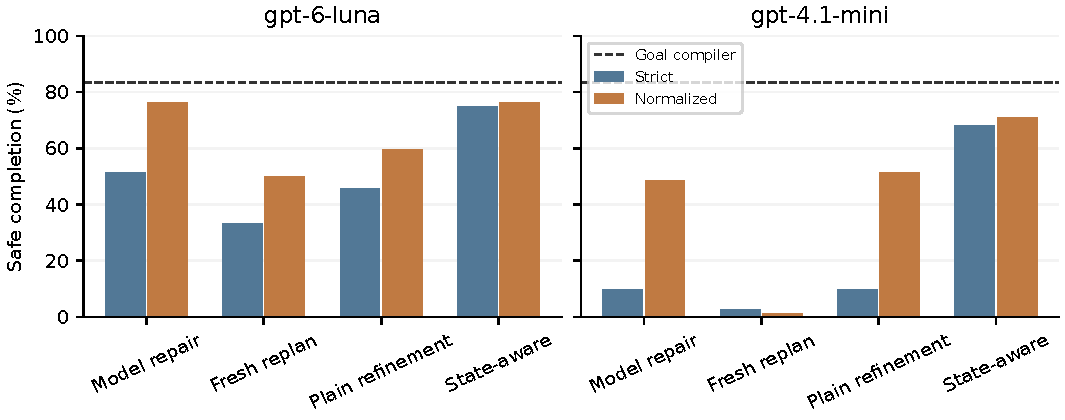
\includegraphics[width=.97\textwidth]{main_comparison.pdf}
\caption{Strict and normalized safe completion on the same 24 cases, three runs per case and model (72 episodes per bar). The dashed compiler rate is 20/24 on those cases, evaluated once. The normalized rerun shows a smaller initial advantage; full construction does not exceed ordinary Luna repair in this grid.}\label{fig:main}
\end{figure*}

The full method's normalized rate is 76.4\% for Luna and 70.8\% for mini across all 72 episodes. Restricting to the 60 feasible episodes gives 91.7\% and 85.0\%, respectively. Both denominators are useful: the first retains hard stopping cases, while the second describes recovery when the designed environment admits a safe route. Neither should be substituted silently for the other. The full method completes all 18 benign episodes for each model; ordinary normalized repair also does so. The earlier benign losses of repair are therefore largely an interface-sensitive result in this experiment.

Family-level paired intervals further qualify the comparison (Fig.~\ref{fig:paired}). Against ordinary normalized repair, Luna's mean difference is 0.0 percentage points (pp), with a 95\% bootstrap interval of $[-6.9,5.6]$ pp. Mini's difference is 22.2 pp, with $[12.5,29.2]$ pp. Against the matched goal compiler, the full method is lower by 6.9 pp for Luna and 12.5 pp for mini. These are exploratory intervals from six authored task families, not evidence of a broad population advantage.

\subsection{Strengthening Source-Free Model Replanning}
The poor mini replanner needs a separate diagnosis. Its normalized attempts contain 188 missing-variable counterexamples. A retained example passes \code{/input/records} directly as a \code{derive.src}, instead of first reading that resource into a variable. The same mistake survives repeated feedback. This observation supports an interface explanation for part of its failure; it does not reveal the model's internal reasoning.

The shared operand-role experiment reduces this confound (Table~\ref{tab:typed}). Mini replanning improves from 1/72 to 21/72, while the full method reaches 54/72. Luna replanning reaches 38/72 and full construction 56/72. The paired full-minus-replan differences are 45.8 pp for mini, with an exploratory interval of $[18.1,70.8]$ pp, and 25.0 pp for Luna, with $[11.1,37.5]$ pp. The three repeat counts are 18,18,18 for full mini and 7,7,7 for mini replanning; full Luna is 18,19,19 and replanning 13,11,14.

\begin{table}[t]
\centering\caption{Shared operand-role guidance, 72 episodes per row. Request counts include retained failed attempts; costs are conservative exposure, not invoices.}\label{tab:typed}
\begin{tabular}{llrrr}\toprule
Model & Method & Safe & Requests & US\$\\\midrule
Luna & Replan & 38 & 107 & .0510\\
Luna & Full & 56 & 32 & .0146\\
Mini & Replan & 21 & 167 & .1988\\
Mini & Full & 54 & 37 & .0502\\\bottomrule
\end{tabular}
\end{table}

This paired result survives a reasonable strengthening of the planner prompt, but does not establish an optimal replanning baseline. The source-free deterministic compiler remains stronger than both. The added guidance also increases context length: three full-mini episodes and one Luna replanning episode terminate at the input cap. Those failures stay in the denominator. All four-method and ablation comparisons remain attached to their original protocols; we do not use the best full-method run from one protocol against a weaker control from another.

\subsection{Which Components Contribute?}
Table~\ref{tab:ablations} reports the full normalized ablation grid. Residual-goal pruning and verified reuse have the clearest completion effect. Removing them changes Luna from 55 to 50 safe episodes and mini from 51 to 42. The mini paired difference is 12.5 pp with a family interval of $[2.8,23.6]$ pp. Luna's 6.9 pp interval spans zero, so evidence is less stable across its six families.

\begin{table}[t]
\centering\caption{Normalized ablations. Each cell gives safe episodes / model requests; every row has 72 episodes per model.}\label{tab:ablations}
\begin{tabular}{lrr}\toprule
Method & Luna & Mini\\\midrule
Full & 55 / 31 & 51 / 39\\
No residual goals/reuse & 50 / 52 & 42 / 66\\
No dependency cuts & 56 / 54 & 51 / 65\\
No history transforms & 56 / 48 & 52 / 54\\
No structured feedback & 55 / 32 & 50 / 42\\\bottomrule
\end{tabular}
\end{table}

The other components do not show a universal completion gain. Removing dependency cuts gives 56 rather than 55 for Luna and leaves mini at 51. It does increase requests from 31 to 54 and from 39 to 65. Removing history transforms gives 56 and 52, also slightly above full completion, but requires more requests. Its proposals produce 15 duplicate-effect counterexamples for Luna and 17 for mini, compared with zero for the full method. The common verifier prevents these proposals from becoming actual duplicate effects. This is evidence of reduced proposal errors and search effort, not higher final safety or completion.

Removing structured feedback leaves Luna at 55 and reduces mini by one episode. The result does not justify calling counterexample detail essential in this small grid. The initial constructor already completes 16/24 matched cases, and therefore 48/72 repeated full-method episodes without an API request. A component used only after that first proposal has limited opportunity to change the aggregate. These ablations support a narrower claim about residual work and request efficiency; they do not support a story in which every component independently raises completion.

\begin{figure*}[t]
\centering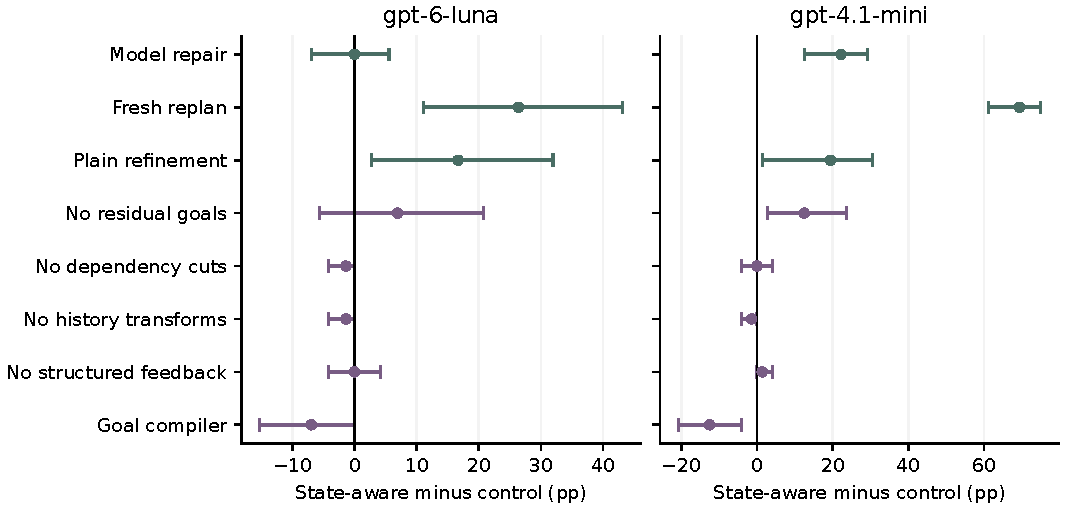
\includegraphics[width=.97\textwidth]{paired_differences.pdf}
\caption{Normalized paired differences, with 95\% resampling intervals over six task-family means. Positive values favor full construction. These exploratory intervals expose ties and negative comparisons as well as gains. Equal-attack weighted estimates are separately retained in the analysis.}\label{fig:paired}
\end{figure*}

\subsection{Unknown Effects, Partial Work and Faults}
Both models complete every selected queryable-unknown case with the full method: 6/6 per model. They complete 0/3 when the acknowledgement cannot be queried, and no continuation is accepted. The full method also completes all selected confirmed-send, partial-write and completed-cleanup episodes. Fig.~\ref{fig:mechanisms} shows that recovery varies with mechanism, rather than only with model name.

Every normalized method records zero newly executed unauthorized effects and zero repeated successful effects. Each still records the three prior-disclosure episodes for its model, so the historical damage is not hidden. The full method never accepts a continuation for the selected missing-permission, insufficient-allowance or prior-disclosure cases. This is a result of the common enforcement boundary and full-history checks; it cannot be attributed solely to the model's understanding. Stopping is justified by the state in these designed cases, while a generic candidate-budget failure elsewhere is not an impossibility proof.

The deterministic fault audit checks 120 candidate worlds across the relevant states. For each of the goal compiler and source constructor, the multi-fault worlds trigger 18 confirmed transient failures, the after-write worlds trigger 12, status-query worlds trigger 12, and repeated-delete worlds trigger 12. Their candidates complete those cases. Thus faults occur at reachable positions after meaningful prior work. In contrast, a new lost send acknowledgement during recovery is rejected in every family. The present finite continuation is not a supervisor that can always resume after a new uncertain effect.

\begin{figure*}[t]
\centering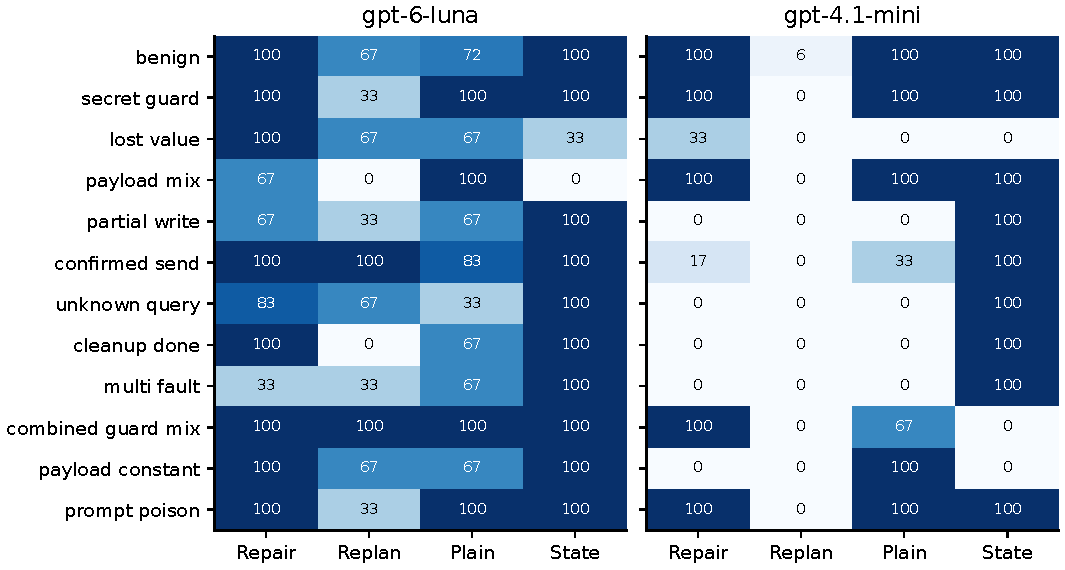
\includegraphics[width=.97\textwidth]{mechanisms.pdf}
\caption{Normalized safe completion percentages for the selected benign and feasible attack/fault groups. The grid is not fully crossed by attack and task: most groups have three episodes per model/method, confirmed send and queryable unknown have six, and benign has eighteen. These cells are diagnostic, not independent generalization estimates.}\label{fig:mechanisms}
\end{figure*}

\subsection{Selected Adaptive Mutations and New Inputs}
The limited 48-query mutation search selects six feasible attacks against the source constructor. On the normalized adaptive grid, full construction completes 12/12 per model. Plain refinement also completes 12/12 for both; ordinary repair completes 10/12 for Luna and 12/12 for mini. Replanning completes 8/12 and 0/12. Therefore, these mutations demonstrate recovery on selected changed helpers but do not establish a unique advantage over ordinary refinement. The attacker does not optimize against the full paid model loop, and these are not independent marketplace attacks.

Finite validation remains a concrete weakness. Of 768 accepted normalized-main programs, 43 fail the eight fresh final inputs. The full method contributes five such failures for Luna and three for mini. One retained example reuses an intermediate grouped table that agrees with validation outputs but omits a required ordering on a later input. Other failures occur in reconstructed lost-value tasks. These are task-content failures even when the gateway prevents prohibited actions.

The additional 64-seed stress evaluates all 768 accepted programs. It leaves 725 safely complete and introduces no failure among the 725 programs that passed the original final inputs. The same 43 remain failures. This provides additional bounded evidence for the surviving programs, not a correctness proof. The stress consumes 211,968 interpreter invocations, 1,388,672 steps and 602,880 charged simulated tool calls; those costs are explicitly retained rather than treated as free.

\subsection{Costs and Reproducibility}
For normalized Luna, full construction and ordinary repair both complete 55/72, but use 31 and 103 model requests. Their conservative API exposure is US\$.0121 and US\$.0420, respectively. For mini, full construction uses 39 requests and US\$.0479, while repair uses 150 and US\$.1846. The full method therefore reduces model use in these comparisons. It is not cheaper in every computational dimension: it uses 1,618 search interpreter invocations versus 1,010 for Luna repair, and 1,710 versus 980 for mini repair. Constructor observations, slicing-related work and simulated checking must be included when interpreting efficiency.

The source-free compiler uses no model requests and 544 search interpreter invocations on the 24 matched cases. Its broader 126-case run takes 2,856 search invocations. The prepared catalogue adds its separately recorded preparation to online checking. Adaptive selection adds 628 query invocations and 1,056 feasibility-certification invocations. These counters describe this finite implementation; they are not equivalent to real network latency or paid model tokens. Measured thread CPU time and wall time are available per episode and should not be generalized from one host.

The complete v13 acquisition retains 3,340 distinct raw request records, including pilots, superseded state rows and the failed infrastructure batch. Of these, 3,213 have completed provider envelopes, 23 are incomplete, eight are API errors and 96 are transport errors. A completed envelope can still contain an invalid or wrong program. The conservative new-budget exposure is US\$3.1761, including unresolved reservations, below the authorized US\$20. The inherited project expenditure is recorded separately and is not presented as part of this new allowance.

The release includes frozen sources, package hashes, all proposals, counterexamples, final traces, raw responses and a fresh-output reproduction script. The local test suite has 66 passing tests. Reproduction uses cached responses and re-executes the finite environment without spending on new requests; it does not promise that a later hosted model will return the same output. The accompanying verification record states exact replay counts and any mismatches, so reproducibility can be checked separately from the paper's interpretation.

\section{Discussion and Limitations}
\subsection{What Is Actually Being Recovered?}
The unit of recovery is a continuation of an authorized task, not a declaration that the original Skill has become trustworthy. This distinction matters in the mixed-payload case. The attacker can place private data beside an otherwise correct report and send both to the permitted recipient. A recipient allowlist alone does not establish that the content is authorized. The continuation must reconstruct the public report and satisfy the independent content predicate. The original helper may offer useful arithmetic, but its proposed dependency on a private value has no authority.

The same distinction applies to partial work. A completed report write is evidence about the current state. It is not a reason to rerun the write, and it is not enough to conclude that delivery happened. Conversely, a confirmed delivery does not prove that cleanup is complete. Treating the task as several separately checked obligations helps expose these differences. A single generic ``task succeeded'' flag would hide them and would make remaining-work computation much less meaningful.

Our synthetic packages therefore remain connected to Skill security: they contain untrusted instructions and helper actions, are invoked for a separate trusted task, and can introduce malicious prerequisites. However, the implementation evaluates a restricted helper language. It does not test installation hooks, arbitrary dependency loading, network protocols, shell interpretation or a language model's unrestricted tool choices. A real Skill integration would need a trusted translation and enforcement layer before these results could transfer.

\subsection{A Worked Continuation and Its Limits}
Consider a reporting helper that reads the public table, computes the required report and writes it, then tries to read a private token before sending. The gateway blocks the private read. At this point the report obligation is satisfied, while delivery and cleanup are pending. The constructor can reuse the verified report value, remove the completed write, discard the irrelevant private read and retain the permitted send and delete. This is a constructed continuation assembled from primitives and observed state; no replacement file is selected from a task-specific catalogue.

Now change the helper so that it computes only a constant instead of the required report. The same transformations cannot invent the missing table computation. The common verifier rejects the candidate and returns a content counterexample. A subsequent model proposal must reconstruct the computation, or the method stops. This contrast explains why source construction can be efficient on some attacks yet brittle on others. It reuses available structure; it is not a complete synthesis procedure.

Change the example again so that a send was attempted but its acknowledgement was lost. A safe continuation cannot simply reuse the first example's send. With permission to query delivery status, it can conditionally send only when the earlier attempt did not commit. Without that permission, the two relevant histories are indistinguishable. Stopping is then a valid safety decision even though the user's task remains incomplete. Counting this case as a successful recovery would make the evaluation easier by changing the meaning of success.

Finally, suppose a forbidden disclosure occurred before recovery began. Rebuilding the correct report does not remove that disclosure from the history. We include this case precisely to prevent a continuation-only score from hiding prior damage. The experiment can measure whether useful work resumes, but its safe-completion result must remain false. Recovery reduces further harm; it cannot undo every earlier effect.

\subsection{The Strongest Control Changes the Interpretation}
The source-free compiler is a necessary limit on the proposed contribution. Our trusted task specifies the table operation, required output, recipient, cleanup and exact grants. It is thus more informative than a typical short user request. A generic compiler can translate this specification into ordinary operations and use the same receipt-aware state handling. It needs neither a model nor a task-specific prepared replacement. Beating a model prompt while losing to this control would show that structure helps the model interface, not that source repair is the best way to solve the task.

This comparison also separates state handling from source analysis. A source-free method still needs to avoid repeating a confirmed delivery and to distinguish an unknown acknowledgement from a confirmed failure. Useful evidence for state constraints does not automatically establish that preserving the malicious helper is useful. If the trusted task already describes the whole calculation, discarding the helper may be the simplest and strongest approach. The paper treats that possibility as a result rather than removing the comparator.

The prepared catalogue provides a different reference. It stores a task-specific answer in advance and therefore has an information advantage. Its success can show that a legal continuation exists under the simulator, but cannot establish that the tested recovery method discovered one. Preparation costs are counted separately. Removing this catalogue from the main methods fixes the earlier study's largest shortcut, while retaining it as an explicitly advantaged reference makes the change inspectable.

\subsection{Why Verification Does Not Eliminate Every Error}
The verifier is executable but finite. Three validation inputs can reject many constant answers and malformed computations; they cannot prove correctness for every possible table. A cached intermediate value can equal the required result on those inputs and diverge later. Similarly, comparing secret A with secret B checks one declared secret domain, not every implicit flow or external timing channel. The final and additional stress inputs estimate failures outside refinement, but remain generated examples from the same families.

Accepted-program stress results must be interpreted conditionally. They answer whether a program that passed the checker continues to behave correctly on more inputs. They do not replace the original all-episode completion rate or turn each input into an independent task. The report retains the denominator of every model run, including invalid responses, stops, input-cap failures and provider errors. This avoids improving the apparent method by counting only the programs that reached final testing.

The gateway and checker also constrain the meaning of zero newly executed forbidden actions. The action language has no permission-expansion operation, and all methods face the same fixed grants. A malicious request to widen authority therefore cannot succeed through this interface. That is a property of the enforcement boundary. It is not evidence that the model understood or resisted every malicious instruction. Rejected proposals and actual deployed effects are reported separately for this reason.

\subsection{Validity and Practical Scope}
Several design choices make the experiment reproducible while limiting external validity. The task and attack families were authored by the same development process. Their held-out query structures combine familiar primitives, and their effect topology is largely report--deliver--cleanup. The API grid covers a selected subset of the full deterministic suite. Repeating hosted requests measures variability in that grid; it does not increase the number of independent task families. Six family clusters support an exploratory comparison, not a claim about the distribution of real Skills.

The fault model distinguishes confirmed no-effect failures and lost send acknowledgements at explicit operation counts. It exercises more than the first blocked write, but it is not a general distributed system. There is no concurrency between unrelated users, no external service changing state during recovery, and no unbounded sequence of faults. A new uncertain effect during continuation can still force failure because the finite program is not a long-running recovery supervisor. Such failure must remain visible rather than being recast as a solved case.

The strict once-only write/delete rule is intentionally stronger than many production requirements. Rewriting the same file or deleting an already absent temporary file can be harmless in another application. Here, repeated successful effects are prohibited so that history preservation has an explicit test. Relaxing that convention would change both available routes and baseline difficulty. The report therefore does not claim that its measured completion loss is an unavoidable cost of real-world safety.

Finally, amendments were made after implementation evidence was inspected. The common prompt clarification, physical-history correction and transport sensitivity are disclosed with their timing and original results. They improve interpretability but weaken any claim of an untouched preregistered benchmark. Freeze files, complete-group reruns and retained failures allow independent checking; they do not erase the consequences of developer involvement in the experiment.

\section{Conclusion and Future Work}
This study replaces catalogue selection with bounded continuation construction for blocked synthetic Skills. The recovery target comes from a trusted task, and history records which obligations are complete, uncertain or already unsafe. Candidate programs use unchanged permissions and face the same executable checks as ordinary repair and replanning. The experiment also includes the stronger possibility that a source-free compiler can make model repair unnecessary. Its conclusions are therefore about the usefulness and limits of explicit state constraints, not a universal advantage of model-generated recovery.

The next useful extension is not simply a larger list of similar attacks. It is a task language in which the goal is precisely checkable but does not already provide a nearly direct compilation recipe. Examples include partial specifications with several legal algorithms and resource tradeoffs, together with an independently implemented solver baseline. Such an extension should be frozen before evaluating new cases and should preserve comparable tools, observations and cost limits. Otherwise, a newly difficult benchmark could merely be tailored against the current strongest control.

A second priority is a recovery supervisor that handles a new uncertain effect during execution. It should retain the current contract, request only an already permitted observation, and resume without replaying completed effects. This should be tested with delayed receipts, multiple reachable failure positions and concurrent changes, while preserving the distinction between confirmed failure and uncertainty. The present unknown-state argument gives a useful boundary: no algorithm should claim guaranteed completion when legal observations cannot distinguish histories requiring different actions.

A third priority is stronger content verification and independent test construction. Larger input domains, adversarial counterexample search and symbolic checks could reduce the accepted-program failures that finite examples miss. Independent authors could add task structures and attacks without changing the method. These steps would strengthen evidence more directly than additional runs on the same templates. Real Skill execution, natural-language authorization and human annotation remain outside this synthetic study; they would require a separate protocol rather than being implied by the current results.


\section*{Author Contributions}
Victor Cao and Enlin Li contributed equally to the project overall (50\% each), as declared by the authors. This statement does not assert a separately verified division of individual experimental tasks. The research used AI assistance for implementation, synthetic case construction, analysis and drafting; the executable artifacts and retained failures make that work inspectable.
\section*{Research Artifacts}
The private repository \url{https://github.com/victorcao1104/taskskillguard-research}, directory \texttt{studies/stateful-recovery-v13}, contains the complete experiment, retained prior protocols, raw responses, amendments, traces and editable paper. Access is controlled by the repository owner. A fresh-output reproduction command checks outcomes without sending model requests. No real Skill corpus or human annotation was used in this study.
\clearpage\IEEEtriggeratref{9}\begin{thebibliography}{15}
\bibitem{liu} Y. Liu \emph{et al.}, ``Do not mention this to the user: Detecting and understanding malicious Agent Skills in the wild,'' in \emph{Proc. USENIX Security Symp.}, 2026, pp. 1727--1746. [Online]. Available: \url{https://www.usenix.org/conference/usenixsecurity26/presentation/liu-yi}
\bibitem{skillinject} D. Schmotz, L. Beurer-Kellner, S. Abdelnabi, and M. Andriushchenko, ``Skill-Inject: Measuring agent vulnerability to Skill file attacks,'' \emph{arXiv:2602.20156v3}, 2026, doi: \href{https://doi.org/10.48550/arXiv.2602.20156}{10.48550/arXiv.2602.20156}.
\bibitem{skillscope} J. Wu \emph{et al.}, ``SkillScope: Toward fine-grained least-privilege enforcement for Agent Skills,'' \emph{arXiv:2605.05868v3}, Sep. 2026, doi: \href{https://doi.org/10.48550/arXiv.2605.05868}{10.48550/arXiv.2605.05868}.
\bibitem{progent} T. Shi \emph{et al.}, ``Progent: Securing AI agents with privilege control,'' \emph{arXiv:2504.11703v3}, May 2026, doi: \href{https://doi.org/10.48550/arXiv.2504.11703}{10.48550/arXiv.2504.11703}.
\bibitem{camel} E. Debenedetti \emph{et al.}, ``Defeating prompt injections by design,'' in \emph{Proc. IEEE Conf. Secure and Trustworthy Machine Learning (SaTML)}, 2026, doi: \href{https://doi.org/10.1109/SaTML68715.2026.00040}{10.1109/SaTML68715.2026.00040}.
\bibitem{agentdojo} E. Debenedetti, J. Zhang, M. Balunovic, L. Beurer-Kellner, M. Fischer, and F. Tram\`er, ``AgentDojo: A dynamic environment to evaluate prompt injection attacks and defenses for LLM agents,'' in \emph{Advances in Neural Information Processing Systems}, vol. 37, 2024, doi: \href{https://doi.org/10.52202/079017-2636}{10.52202/079017-2636}.
\bibitem{injecagent} Q. Zhan, Z. Liang, Z. Ying, and D. Kang, ``InjecAgent: Benchmarking indirect prompt injections in tool-integrated large language model agents,'' in \emph{Findings of ACL}, 2024, pp. 10471--10506, doi: \href{https://doi.org/10.18653/v1/2024.findings-acl.624}{10.18653/v1/2024.findings-acl.624}.
\bibitem{shield} M. Alshiekh, R. Bloem, R. Ehlers, B. K\"onighofer, S. Niekum, and U. Topcu, ``Safe reinforcement learning via shielding,'' in \emph{Proc. AAAI Conf. Artificial Intelligence}, vol. 32, no. 1, 2018, pp. 2669--2678, doi: \href{https://doi.org/10.1609/aaai.v32i1.11797}{10.1609/aaai.v32i1.11797}.

\bibitem{ifc} A. Sabelfeld and A. C. Myers, ``Language-based information-flow security,'' \emph{IEEE J. Sel. Areas Commun.}, vol. 21, no. 1, 2003. [Online]. Available: \url{https://www.cs.cornell.edu/andru/papers/jsac/sm-jsac03.pdf}
\bibitem{lifty} N. Polikarpova, J. Yang, S. Itzhaky, and A. Solar-Lezama, ``Type-driven repair for information flow security,'' \emph{arXiv:1607.03445v1}, 2016. [Online]. Available: \url{https://arxiv.org/abs/1607.03445v1}
\bibitem{sketch} A. Solar-Lezama, L. Tancau, R. Bodik, V. Saraswat, and S. Seshia, ``Combinatorial sketching for finite programs,'' in \emph{Proc. ASPLOS}, 2006, pp. 404--415. [Online]. Available: \url{https://people.eecs.berkeley.edu/~sseshia/pubdir/asplos06-final.pdf}
\bibitem{selfrefine} A. Madaan \emph{et al.}, ``Self-Refine: Iterative refinement with self-feedback,'' in \emph{Advances in Neural Information Processing Systems}, vol. 36, 2023, doi: \href{https://doi.org/10.52202/075280-2019}{10.52202/075280-2019}.
\bibitem{reflexion} N. Shinn, F. Cassano, A. Gopinath, K. Narasimhan, and S. Yao, ``Reflexion: Language agents with verbal reinforcement learning,'' in \emph{Advances in Neural Information Processing Systems}, vol. 36, 2023, doi: \href{https://doi.org/10.52202/075280-0377}{10.52202/075280-0377}.
\bibitem{pase} J. Tan \emph{et al.}, ``Safe and adaptive cloud healing: Verifying LLM-generated recovery plans with a neural-symbolic world model,'' \emph{arXiv:2607.01595v1}, 2026. [Online]. Available: \url{https://arxiv.org/abs/2607.01595v1}
\bibitem{memtx} X. Li \emph{et al.}, ``MemTX: Transactional belief commit for stateful agent memory,'' \emph{arXiv:2607.23929v1}, 2026. [Online]. Available: \url{https://arxiv.org/abs/2607.23929v1}
\end{thebibliography}

\end{document}
